\documentclass[tikz, border=10pt]{standalone}
\usepackage{iftex}
\ifluatex
  \usepackage{fontspec}
  \usepackage{unicode-math}
  \setmainfont{Fira Sans}
  \setmonofont{Fira Mono}
  \setmathfont{Fira Math}
  \setmathfont{STIX Two Math}[range={"29F5,"2216}]
\else
  \usepackage[T1]{fontenc}
\fi

\usepackage{amsmath}
\usepackage{tikz}
\usetikzlibrary{arrows.meta}
\tikzset{every node/.style={font=\Large}}

% Theme toggle: \darkbgfalse for light background preview.
\newif\ifdarkbg
\darkbgfalse
\ifdarkbg
  \colorlet{axiscol}{white}
  \colorlet{gridcol}{white!30!black}
  \colorlet{ticklabelcol}{white}
  \colorlet{funcol}{yellow!85!white}
\else
  \colorlet{axiscol}{black}
  \colorlet{gridcol}{black!25!white}
  \colorlet{ticklabelcol}{black}
  \colorlet{funcol}{blue!70!black}
\fi

% x: -4 to 6  (10 units)  xscale=0.80 → ~8.0 cm wide
% y: -3 to  1  ( 4 units)  yscale=1.30 → ~5.2 cm tall
% Domain starts at x = -3.  f(6) = -3 → exits at exact corner.
% Integer points: (-3,0)  (-2,-1)  (1,-2)  (6,-3)
\begin{document}
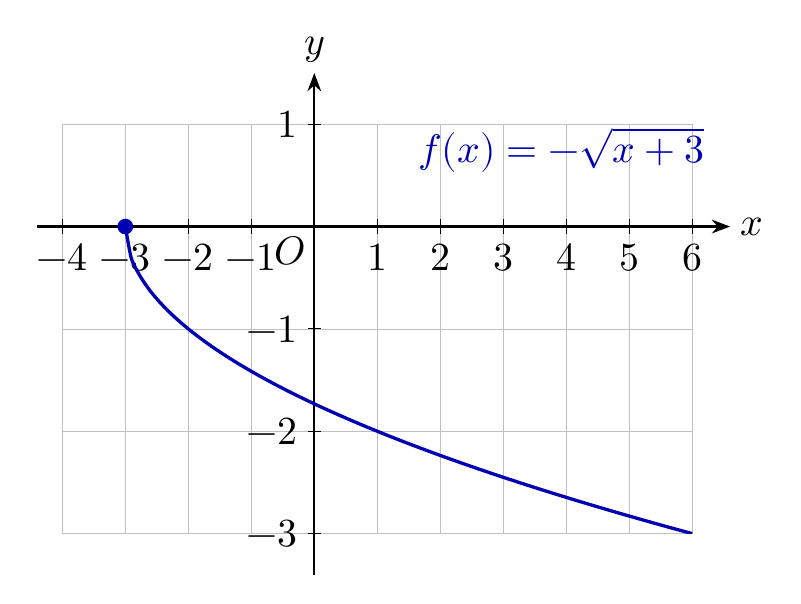
\begin{tikzpicture}[xscale=0.80, yscale=1.30, >=Stealth]

  % Cartesian grid.
  \draw[step=1, very thin, gridcol] (-4,-3) grid (6,1);

  % Axes.
  \draw[->, thick, axiscol] (-4.4,0) -- (6.6,0)
    node[right, text=axiscol] {$x$};
  \draw[->, thick, axiscol] (0,-3.4) -- (0,1.5)
    node[above, text=axiscol] {$y$};

  % Tick marks — x axis (every 1).
  \foreach \x in {-4,-3,-2,-1,1,2,3,4,5,6} {
    \draw[axiscol] (\x, 2pt) -- (\x, -2pt)
      node[below, text=ticklabelcol] {$\x$};
  }

  % Tick marks — y axis (every 1).
  \foreach \y in {-3,-2,-1,1} {
    \draw[axiscol] (3pt,\y) -- (-3pt,\y)
      node[left, text=ticklabelcol] {$\y$};
  }

  % Origin label.
  \node[below left, text=axiscol] at (0,0) {$O$};

  % Function curve: f(x) = -sqrt(x+3), domain x >= -3.
  \begin{scope}
    \clip (-4,-3) rectangle (6,1);
    \draw[domain=-3:6, smooth, very thick, funcol, samples=100]
      plot (\x, {-sqrt(\x+3)});
  \end{scope}

  % Function label — upper right, above the curve.
  \node[right, text=funcol] at (1.5,0.75) {$f(x)=-\sqrt{x+3}$};

  % Key points.
  \node[circle, fill=funcol, inner sep=2pt] at (-3,0)  {};  % domain start
  % \node[circle, fill=funcol, inner sep=2pt] at (-2,-1) {};
  % \node[circle, fill=funcol, inner sep=2pt] at (1,-2)  {};
  % \node[circle, fill=funcol, inner sep=2pt] at (6,-3)  {};  % corner exit

\end{tikzpicture}
\end{document}
